\chapter{Results}

\section{Prompt Pairs}

\begin{figure}
    \centering
    \captionsetup{width=.9\textwidth}
    \begin{subfigure}{0.52\textwidth}
        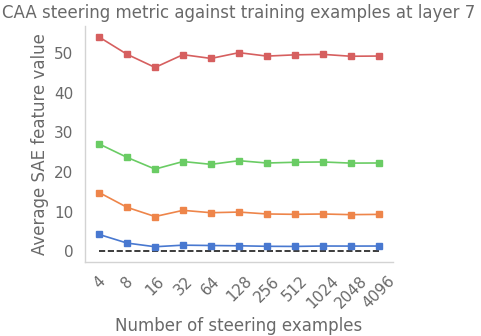
\includegraphics[width=\textwidth]{figures/prompt_pairs_caa_1.png}
        \caption{ }
    \end{subfigure}
    \begin{subfigure}{0.43\textwidth}
        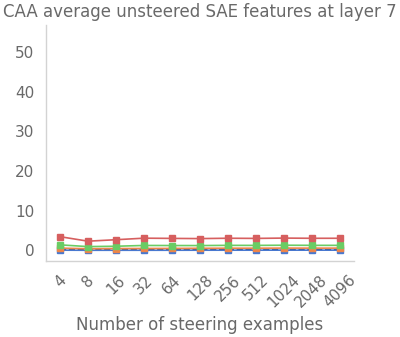
\includegraphics[width=\textwidth]{figures/prompt_pairs_caa_2.png}
        \caption{ }
    \end{subfigure}
    \begin{subfigure}{0.45\textwidth}
        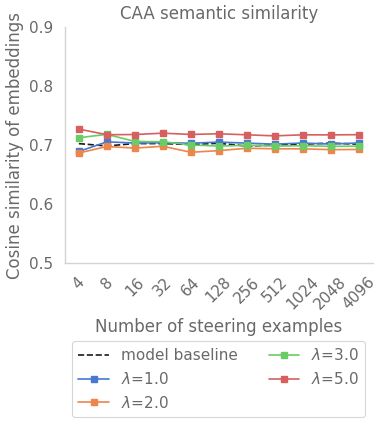
\includegraphics[width=\textwidth]{figures/prompt_pairs_caa_3.png}
        \caption{ }
    \end{subfigure}
    \caption{Result of running CAA \citep{caa} in the prompt pairs environment \Sref{sec:prompt-pairs} on GPT2 at layer 7. (a) The average activation of the target SAE features. (b) The average activation of SAE features that were not present in the positive or negative examples. (c) The semantic similarity of the generated token and the target token. In all cases the dashed line is the baseline for the model without steering.}
    \label{fig:gpt_pp_caa}
\end{figure}

